\documentclass[10pt,a4paper]{article}
\usepackage[utf8]{inputenc}
\usepackage{amsmath}
\usepackage{gensymb}
\usepackage{amsfonts}
\usepackage{siunitx}
\usepackage[european]{circuitikz}
\usepackage{geometry}
\newgeometry{tmargin=2cm, bmargin=2cm, lmargin=2cm, rmargin=2cm}
\usepackage{amssymb}
\usepackage{polski}
\usepackage{graphicx}
\author{\textbf{T. Fąs}}
\title{\textbf{ABSORPCJA ŚWIATŁA W MATERII}}
\begin{document}
\maketitle

\begin{center}
\textbf{\subsection*{STRESZCZENIE}}
\end{center}
Celem doświadczenia było wyznaczenie współczynnika absorpcji $\alpha$ dla badanego ciała, związanej z nim średniej drogi swobodnej fotonu $\lambda$, znalezienie zależności grubości filtra $L$ od absorbancji $A$ oraz znalezienie zależności absorbancji od grubości filtra, absorbancji od stężenia roztworu CuSO$_{4}$ i współczynnika odbicia $R$. Wyznaczono $\alpha=0,5735\pm0,0019$ mm$^{-1}$, $\lambda=1,7437\pm0,0058$ mm, $R=0,05 \pm 0,28$, $A(L)=\hat{a}L+\hat{b}$; dla pojedynczych filtrów: $\hat{a}=0,2478\pm0,0016$ mm$^{-1}$, $\hat{b}=0,040\pm0,0058$, dla filtrów podwójnych: $\hat{a}=0,24954\pm0,00098$ mm$^{-1}$, $\hat{b}=0,0603\pm0,0073$, dla układu trzech filtrów: $\hat{a}=0,168\pm0,045$ mm$^{-1}$, $\hat{b}=1,28\pm0,68$. Dla roztworu dane nie przeszły testu $\chi^2$ Pearsona. Zależność odwrotna jest dana wzorem: $L(A)=\hat{\alpha}A+\hat{\beta}$, gdzie $\hat{\alpha}=4,035\pm0,026$ mm, $\hat{\beta}=-0,162\pm0,024$ mm.


\begin{center}
\textbf{\subsection*{WSTĘP}}
\end{center}
Zgodnie z korpuskularnym podejściem do natury światła, jego natężenie po przejściu przez ośrodek o grubości $L$ i  współczynniku absorpcji $\alpha$ wynosi:
\begin{equation}
I(L)=I_{0}\exp(-\alpha L),
\end{equation}
gdzie $I_{0}$ jest pierwotnym natężeniem światła. W przypadku roztworów współczynnik $\alpha$ można przedstawić jako $\alpha=\varepsilon c$, gdzie $\varepsilon$ jest molowym współczynnikiem absorpcji, a $c$ jest stężeniem molowym danego roztworu. W przypadku rzeczywistym należy wziąć pod uwagę efekt odbicia światła od powierzchni materiału, jak i również należy ustalić sposób badania natężenia światła, stąd też wygodnie jest badać tak zwany współczynnik transmisji dany wzorem;
\begin{equation}
T=\frac{I_{T}(L)}{I_{0}}=(1-R)^2\exp(-\alpha L),
\end{equation}
gdzie $R$ jest współczynnikiem odbicia danego materiału, a $I_{T}(L)$ jest natężeniem światła po przejściu przez materiał wraz z uwzględnieniem odbicia \cite{sz1}.

Jednak w pracy eksperymentalnej taka postać jest ciężka w analizie, stąd też postanowiono wprowadzić zależność:
\begin{equation}
I(L)=I_{0}10^{-A},
\end{equation}
gdzie wielkość $A$ zwana jest absorbancją. Łącząc Równanie (3) z Równaniem (2) i tworząc z nich równanie liniowe, otrzymano:
\begin{equation}
A=-\log_{10}(T)=\alpha L\log_{10}(e)-2\log_{10}(1-R).
\end{equation}
W ten sposób otrzymano łatwą w analizie zależność, która pozwala na wyznaczenie współczynnika $\alpha$ oraz $R$. 
W przypadku $n$ warstw tego samego materiału o różnej grubości, Równanie (4) można uogólnić do postaci:
\begin{equation}
A=\alpha\log_{10}(e)(L_{1}+L_{2}\ldots+L_{n})-2n\log_{10}(1-R).
\end{equation}
\begin{center}
\textbf{\subsection*{UKŁAD DOŚWIADCZALNY}}
\end{center}
Układ doświadczalny składał się z lasera, sześciu filtrów wykonanych z tego samego materiału, o różnej grubości, fotodiody, woltomierza, rynny, kuwety, wody destylowanej, strzykawki, pipety i roztworu CuSO$_{4}$ o stężeniu molowym 1,157 mol/L. 

Laser i fotodioda były ustawione na przeciwnych krańcach rynny tak, że laser trafia w środek fotodiody. Bezpośrednio przed fotodiodą ustawiano filtry. Do fotodiody był podłączony woltomierz, którego zakres zmieniano ręcznie, w zależności od aktualnego napięcia. Całość pomiarów była przeprowadzana w ciemnym pomieszczeniu. Wykonano pomiary napięcia na fotodiodzie dla pojedynczych filtrów oraz różnych kombinacji dwóch oraz trzech filtrów. W przypadku roztworu CuSO$_{4}$ kuwetę ustawiono tuż przed laserem. W pierwszej fazie pomiarów do kuwety nalano 1 ml wody destylowanej i dolewano po 0,1 ml roztworu. Napięcie mierzono przy każdym dolaniu. W drugiej fazie najpierw nalano 1 ml roztworu do kuwety, a następnie dolewano po 0,2 ml wody destylowanej. 

\begin{center}
\textbf{\subsection*{WYNIKI POMIARÓW}}
\end{center}
Wykorzystano filtry z zestawu A o oznaczeniach i grubościach $L$ przedstawionych w Tabeli 1. Pomiary dla pojedynczych filtrów z tego zestawu prezentuje Tabela 2. Kolumna "Zakres" informuje, jaki był zakres woltomierza w momencie wykonywania pomiaru.


\begin{table}[h!]
\centering
\caption{Oznaczenia i grubości filtrów}
\label{t1}
\begin{tabular}{|c|c|c|c|c|c|c|}
\hline
Oznaczenie & A1    & A2    & A3    & A4    & A5    & A6    \\ \hline
L [mm]     & 1,040 & 2,510 & 3,876 & 4,832 & 6,577 & 7,704 \\ \hline
\end{tabular}
\end{table}

\begin{table}[h!]
\centering
\caption{Pomiary: pojedynczy filtr}
\label{t2}
\begin{tabular}{|c|c|c|}
\hline
U [V] & Filtr & Zakres \\ \hline
6,69  & brak     & 20 V   \\ \hline
0,144 & A5    & 2 V    \\ \hline
0,075 & A6    & 2 V    \\ \hline
0,390 & A4    & 2 V    \\ \hline
0,662 & A3    & 2 V    \\ \hline
1,450 & A2    & 2 V    \\ \hline
3,40  & A1    & 20 V   \\ \hline
\end{tabular}
\end{table}


Pomiary dla zestawu dwóch i trzech filtrów prezentują kolejno Tabela 3 i Tabela 4. 

\begin{table}[h!]

\setlength\tabcolsep{4 pt}
\begin{minipage}{0.5\textwidth}
\centering
\caption{Pomiary: dwa filtry}
\begin{tabular}{|c|c|c|}
\hline
U [V]  & Filtr & Zakres \\ \hline
0,7530 & A1+A2 & 2 V    \\ \hline
0,0084 & A5+A4 & 200 mV \\ \hline
0,0073 & A6+A3 & 200 mv \\ \hline
0,0165 & A2+A6 & 200 mv \\ \hline
0,2030 & A1+A4 & 2 V    \\ \hline
0,7400 & A1+A5 & 2 V    \\ \hline
0,0144 & A3+A5 & 200 mV \\ \hline
\end{tabular}


\end{minipage}
\hfill
\begin{minipage}{0.5\textwidth}
\centering
\caption{Pomiary: trzy filtry}
\begin{tabular}{|c|c|c|}
\hline
U [V]  & Filtr    & Zakres \\ \hline
0,0074 & A1+A3+A5 & 2 V    \\ \hline
0,0039 & A1+A5+A6 & 200 mV \\ \hline
0,0019 & A2+A3+A4 & 200 mv \\ \hline
0,0002 & A3+A5+A6 & 200 mv \\ \hline
\end{tabular}
\end{minipage}
\end{table}

Wyniki pomiarów dla roztworu CuSO$_{4}$ o stężeniu $c$ przedstawia Tabela 5.

\begin{table}[h!]
\centering
\caption{Pomiary: roztwór CuSO$_{4}$}
\label{t5}
\begin{tabular}{|c|c|c||c|c|c|}
\hline
U [V]  & c [mol/L] & Zakres & U [V]  & c [mol/L] & Zakres \\ \hline
5,8    & 0,00000   & 20 V   & 0,1395 & 0,57850   & 200 mV \\ \hline
2,64   & 0,10518   & 20 V   & 0,1175 & 0,60605   & 200 mV \\ \hline
0,709  & 0,33057   & 2 V    & 0,0144 & 1,15700   & 200 mV \\ \hline
0,432  & 0,38567   & 2 V    & 0,0103 & 0,89000   & 200 mV \\ \hline
0,341  & 0,43388   & 2 V    & 0,0384 & 0,77133   & 200 mV \\ \hline
0,224  & 0,47641   & 2 V    & 0,0428 & 0,68059   & 200 mV \\ \hline
0,201  & 0,51422   & 2 V    & 0,0455 & 0,60895   & 200 mV \\ \hline
0,1808 & 0,54805   & 200 mV & 0,0502 & 0,55095   & 200 mV \\ \hline
\end{tabular}
\end{table}
Warto nadmienić, iż laser nie był poprawnie wykalibrowany i wiązka światła nie trafiała w środek fotodiody. Prawidłowa kalibracja okazała się niestabilna, co zaburzyło końcowe pomiary. Dodatkowo otrzymana kuweta była porysowana, co miało istotny wpływ na wyniki. Innym aspektem zaburzającym pomiary były strzykawki, które stawiały opór przy dolewaniu roztworu, przez co niemożliwe było precyzyjne dawkowanie cieczy. W efekcie pomiary związane z roztworem CuSO$_{4}$ są obarczone ogromnym błędem pomiarowym.



\begin{center}
\textbf{\subsection*{ANALIZA DANYCH}}
\end{center}
Aby przeprowadzić analizę zebranych danych, należy w pierwszej kolejności poznać niepewności związane z pomiarem napięcia. W tym celu posłużono się instrukcją dołączoną przez producenta i przedstawioną na Rysunku 1. Korzystając z zawartych tam informacji obliczono niepewności dla zestawu danych z Tabeli 2 i przedstawiono je w Tabeli 6.

\begin{figure}[h!]
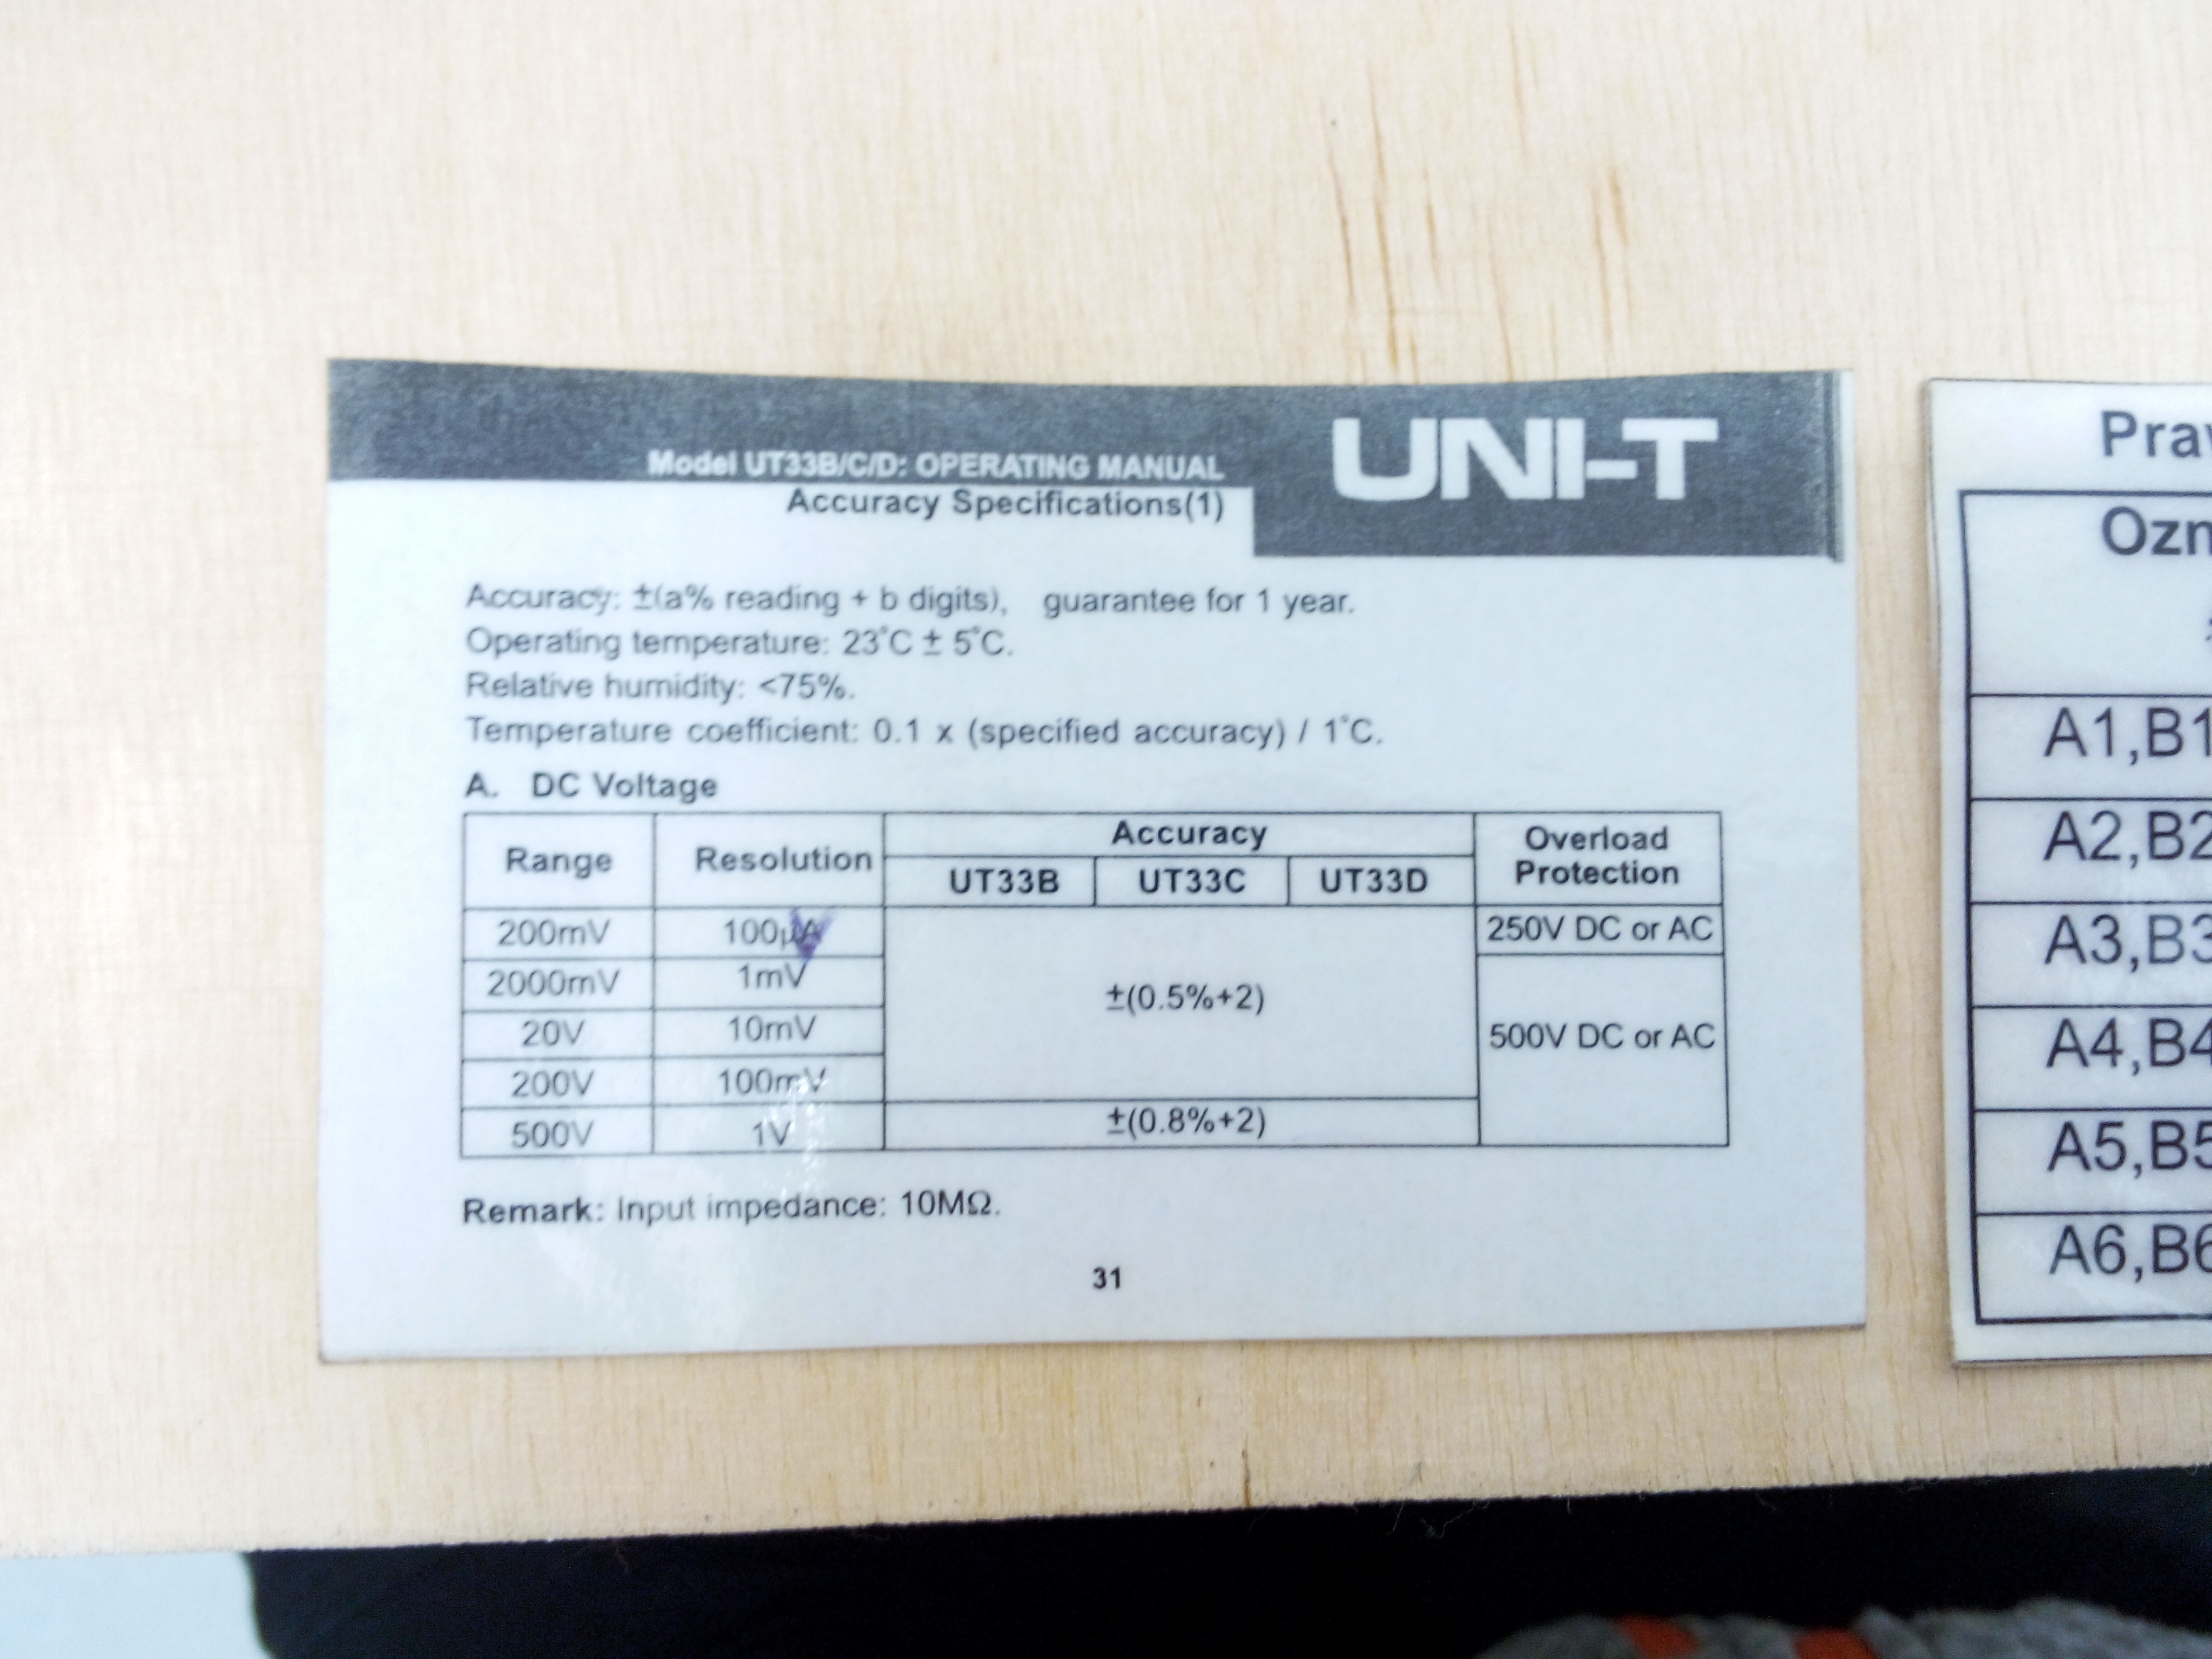
\includegraphics[width=10cm]{rap7} 
\centering
\caption{Niepewności pomiaru napięcia.}
\end{figure}

 Kolejnym krokiem było obliczenie wartości absorbancji, która w tym przypadku jest zdefiniowana jako:
\begin{equation}
A=\log_{10}\left(\dfrac{U}{U_{0}}\right),
\end{equation}
gdzie $U_{0}$ jest napięciem zmierzonym bez żadnego filtra. Zastosowanie napięcia zamiast natężenia światła jest uzasadnione tym, że mierzone napięcie jest wprost proporcjonalne do natężenia światła. Niepewność absorbancji obliczono, korzystając z metody propagacji małych błędów, wyrażającej się wzorem:
 \begin{equation}
 u_{f}^2=\sum_{i=1}^n \left( \dfrac{\partial f}{\partial x_{i}}u_{i}\right)^2+\sum_{i=1, i\neq j}^n \left( \dfrac{\partial f}{\partial x_{i}}\dfrac{\partial f}{\partial x_{j}}c_{ij}\right),
 \end{equation}
 gdzie wielkość $f$ zależy od wielkości $x_{i}$ o niepewnościach $u_{i}$ i o ocenach kowariancji $c_{ij}$. W przypadku mierzonych napięć, kowariancja między nimi wynosi 0. Zastosowanie Równania (7) do Równania (6) prowadzi do wyniku:
 \begin{equation}
 u_{A}=\dfrac{1}{\ln(10)}\sqrt{\dfrac{u_{U_{0}}^2}{U_{0}^2}+\dfrac{u_{U_{n}}^2}{U_{n}^2}}
\end{equation}
Wyniki oparte na Równaniu (8) również umieszczono w Tabeli 6.

\begin{table}[h!]
\centering
\caption{Niepewności napięcia; absorbancja i jej niepewności}
\label{t6}
\begin{tabular}{|c|c|c|c|}
\hline
U [V] & $u_{U}$ [V] & A       & $u_{A}$ \\ \hline
0,144 & 0,00272     & 1,66706 & 0,00891 \\ \hline
0,075 & 0,00238     & 1,95036 & 0,01418 \\ \hline
0,39  & 0,00395     & 1,23436 & 0,00560 \\ \hline
0,662 & 0,00531     & 1,00457 & 0,00492 \\ \hline
1,45  & 0,00925     & 0,66406 & 0,00444 \\ \hline
3,4   & 0,03700     & 0,29395 & 0,00586 \\ \hline
\end{tabular}
\end{table}

Zgodnie z Równaniem (4) dane te podlegają zależności liniowej postaci $A=\hat{a}L+\hat{b}$. Aby wyznaczyć najlepsze oceny parametrów $\hat{a}$ i $\hat{b}$ posłużono się metodą najmniejszych kwadratów. Polega ona na minimalizacji wielkości, która w tym przypadku dana jest wzorem;
\begin{equation}
R\left(\hat{a}, \hat{b} \right)=\sum_{i=1}^{5}\left(\dfrac{A_{i}-\hat{a}L_{i}-\hat{b}}{u_{Ai}}\right)^2 \quad \cite{tay1}
\end{equation}
W trakcie trakcie dopasowywania krzywej najlepszego dopasowania celowo pominięto jeden punkt: ten związany z filtrem A6, aby móc użyć go później jako wzorca dla zależności odwrotnej. 

Po podstawieniu odpowiednich wartości do Równania (9) otrzymano: $\hat{a}=0,2478\pm0,0016$ mm$^{-1}$, $\hat{b}=0,040\pm0,0058$, z kowariancją $c_{ab}=-0,0000083$ mm$^{-1}$, wraz z oceną tej kowariancji $\rho=-0,90637$. Jak widać, ocena kowariancji wskazuje na silną zależność liniową między $\hat{a}$ i $\hat{b}$, choć sama wartość kowariancji jest bardzo mała. 

Aby zyskać pewność, co do przyjętego modelu teoretycznego, przeprowadzono test $\chi^2$ Pearsona. Polega on na sprawdzeniu, czy wartość $\chi_{0}^2$, wynikająca z ocen parametrów, jest mniejsza od wartości krytycznej $\chi^2$ wynikającej z modelu. Wartość $\chi^2$ zależy od ilości stopni swobody oraz od prawdopodobieństwa popełnienia błędu I rodzaju, czyli odrzucenia hipotezy prawdziwej. Na potrzeby tego testu przyjęto prawdopodobieństwo na poziomie $P=0,005$. Ilość stopni swobody to różnica pomiędzy ilością wykonanych pomiarów a liczbą parametrów. W tym przypadku liczba pomiarów wynosi 5, a liczba parametrów jest równa 2. Tak więc liczba stopni swobody wynosi $\nu=5-2=3$. Wartość krytyczną $\chi^2=12,84$ odczytano z tablic statystycznych \cite{g1}. Aby wyznaczyć wartość $\chi_{0}^2$ posłużono się wzorem:
\begin{equation}
 \chi_{0}^2=\sum_{i=1}^N\dfrac{(y_{i}-\hat{a}x-\hat{b})^2}{u_{i}^2} \quad \cite{tay3},
 \end{equation} 
który dla rozpatrywanego przypadku przyjmuje postać:
\begin{equation}
\label{r17}
 \chi_{0}^2=\sum_{i=1}^5\dfrac{(A_{i}-\hat{a}L_{i}-\hat{b})^2}{u_{i}^2} 
 \end{equation} 
Otrzymano wartość $\chi_{0}^2=1,70<12,84$, tak więc wykonane pomiary nie przeczą tezie o liniowej zależności między absorbancją i grubością materiału. Wykres zależności $A(L)$ wraz z krzywą najlepszego dopasowania przedstawia Rysunek 2.

\begin{figure}[h!]
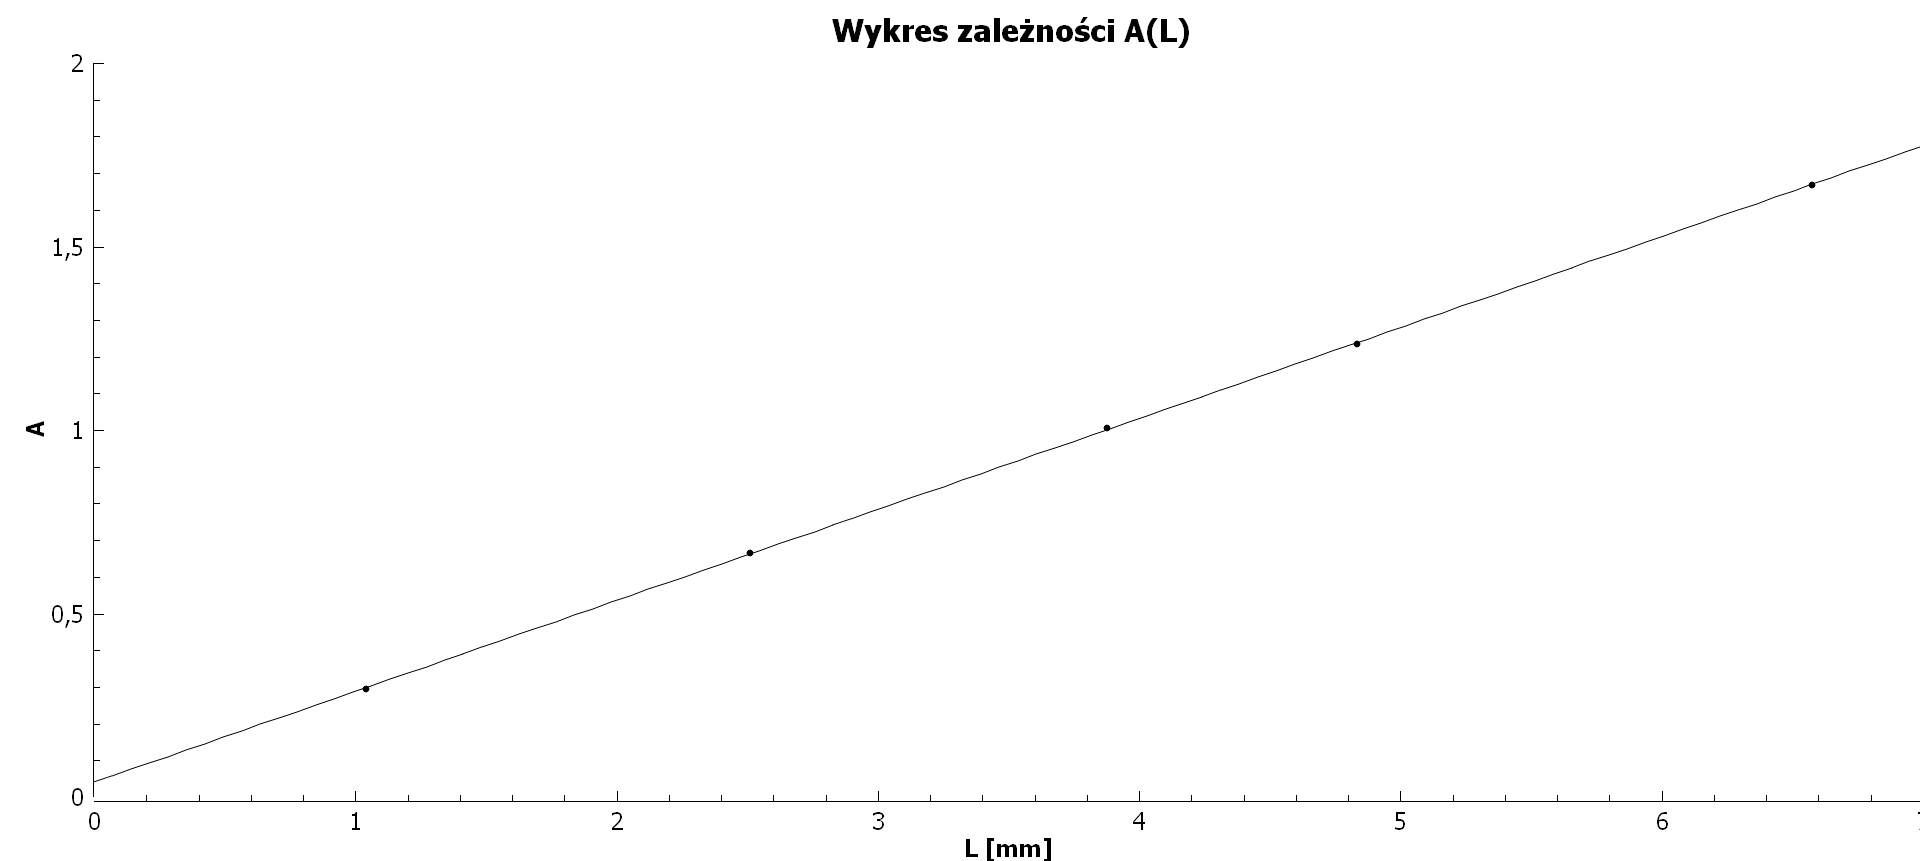
\includegraphics[width=15cm]{rap7rys1} 
\centering
\caption{Wykres zależności A(L)}
\end{figure}

Korzystając z zależności $\hat{b}=-2\log_{10}(1-R)$ obliczono wartość współczynnika odbicia $R$, a jego niepewność obliczono, korzystając z Równania (7). 
\[R=10^{{-b}/{2}}\]
\[u_{R}=\dfrac{2u_{b}}{b} 10^{{-b}/{2}}\]
Otrzymano $R=0,05\pm0,28$. Jak widać, niepewność jest znacznie większa od wartości współczynnika, więc ciężko jest ocenić jego właściwą wartość.


W dalszej analizie danych postanowiono odwrócić zależność $A(L)$, aby otrzymać zależność $L(A)$ wraz z oceną jej niepewności. Otrzymano równanie:
\begin{equation}
L(A)=\dfrac{1}{\hat{a}}A-\dfrac{\hat{b}}{\hat{a}}=\hat{\alpha}A+\hat{\beta},
\end{equation}
przy czym niepewność tego wyrażenia obliczono, korzystając z Równania (7):
\begin{equation}
u_{L}^2=\dfrac{1}{\hat{a}^2}\left(L^{2}u_{\hat{a}}^{2}+2Lc_{ab}+u_{L}^{2}+u_{A}^{2}\right)
\end{equation}
Niepewności wielkości $\hat{\alpha}$i $\hat{\beta}$ również otrzymano, korzystając z Równania (7).
\[u_{\alpha}=\dfrac{u_{\hat{a}}}{\hat{a}^2} \] 
\[ u_{\beta}=\dfrac{\hat{b}}{\hat{a}}\sqrt{\dfrac{u_{\hat{a}}^2}{\hat{a}^2}+\dfrac{u_{\hat{b}^2}}{\hat{b}^2}-\dfrac{2c_{ab}}{ab}}\]

 Otrzymano: $\hat{\alpha}=4,035\pm0,026$ mm, $\hat{\beta}=-0,162\pm0,024$ mm. W następnym kroku wykorzystano pominięty punkt, aby móc określić dokładność zależności $L(A)$. Podstawienie wartości $A=1,95036$ do Równania (12) i Równania (13) zwraca wielkość $L_{o}=7,708\pm0,064$ mm. Różnica pomiędzy otrzymaną wartością, a wartością wzorcową $L=7,704$ mm wynosi 0,004 mm. Aby się przekonać, czy otrzymana wartości $L_{o}$ w porównaniu ze wzorcową są ze sobą zgodne, przeprowadzono test $3\sigma$. Polega on na sprawdzeniu, czy moduł różnicy $|L_{o}-L|$ jest mniejszy od trzykrotności niepewności tej różnicy. Gołym okiem widać, że jest zdecydowanie mniejszy, tak więc wielkości te są ze sobą zgodne.
 
 Przeprowadzono analogiczne rozumowanie i obliczenia w przypadku pomiarów z dwoma filtrami. W tym przypadku otrzymano współczynnik $\hat{b}<0$, co prowadzi do wniosku, iż $R<0$. Jest to oczywista sprzeczność i z tego powodu postanowiono odrzucić punkt z największym odstępstwem od krzywej najlepszego dopasowania, czyli punkt związany z filtrami A1+A5. Ostateczne punkty związane z tą analizą przedstawiono w Tabeli 7.
 
\begin{table}[h!]
\centering
\caption{Punkty pomiarowe: dwa filtry}
\label{my-label}
\begin{tabular}{|c|c|c|}
\hline
$L$ [mm] & $A$     & $u_{A}$ \\ \hline
3,55     & 0,94863 & 0,00481 \\ \hline
11,409   & 2,90115 & 0,01298 \\ \hline
11,536   & 2,96210 & 0,01449 \\ \hline
10,214   & 2,60794 & 0,00821 \\ \hline
5,872    & 1,51793 & 0,00732 \\ \hline
10,453   & 2,66706 & 0,00891 \\ \hline
\end{tabular}
\end{table} 
 Przy czym grubość $L$ jest sumą grubości filtrów wykorzystanych w danym pomiarze. 
 
 Otrzymano następujące wartości parametrów: $\hat{a_{2}}=0,24954\pm0,00098$ mm$^{-1}$, $\hat{b_{2}}=0,0603\pm0,0073$, z kowariancją $c_{ab2}=-0,0000064$ mm$^{-1}$, i oceną tej kowariancji $\rho=-0,90028$ 
 W tym przypadku wykorzystano 6 punktów pomiarowych, więc wartość $\chi^2$ wynosi 14,86. Wartość $\chi_{0}^2$, obliczona zgodnie z Równaniem (11) wynosi 4,18, tak więc otrzymane wyniki nie są sprzeczne z tezą o liniowej zależności $A$ i $L$. 
 
 Dla przypadku trzech wykorzystano punkty przedstawione w Tabeli 8. 
 
 \begin{table}[h!]
\centering
\caption{Punkty pomiarowe: trzy filtry}
\label{t8}
\begin{tabular}{|c|c|c|}
\hline
$L$ [mm] & $A$     & $u_{A}$ \\ \hline
11,493   & 2,95619 & 2,95619 \\ \hline
15,321   & 3,23436 & 3,23436 \\ \hline
11,218   & 3,54667 & 3,54667 \\ \hline
18,157   & 4,52440 & 4,52440 \\ \hline
\end{tabular}
\end{table}
Otrzymano wartości: $\hat{a_{3}}=0,168\pm0,045$ mm$^{-1}$, $\hat{b_{3}}=1,28\pm0,68$, przy czym $\chi_{0}^2=7,19$, co jest mniejsze od wartości $\chi^2=10,60$, tak więc dane te również nie są sprzeczne z hipotezą. Dodatkowo obliczono kowariancję $c_{ab3}=-0,030$ mm$^{-1}$ wraz z oceną $\rho=-0,98$. Wykresy wraz z krzywą najlepszego dopasowania dla dwóch i trzech filtrów przedstawiają Rysunek 3 i Rysunek 4.

\begin{figure}[h!]
\centering
\begin{minipage}{0.5\textwidth}
  \centering
  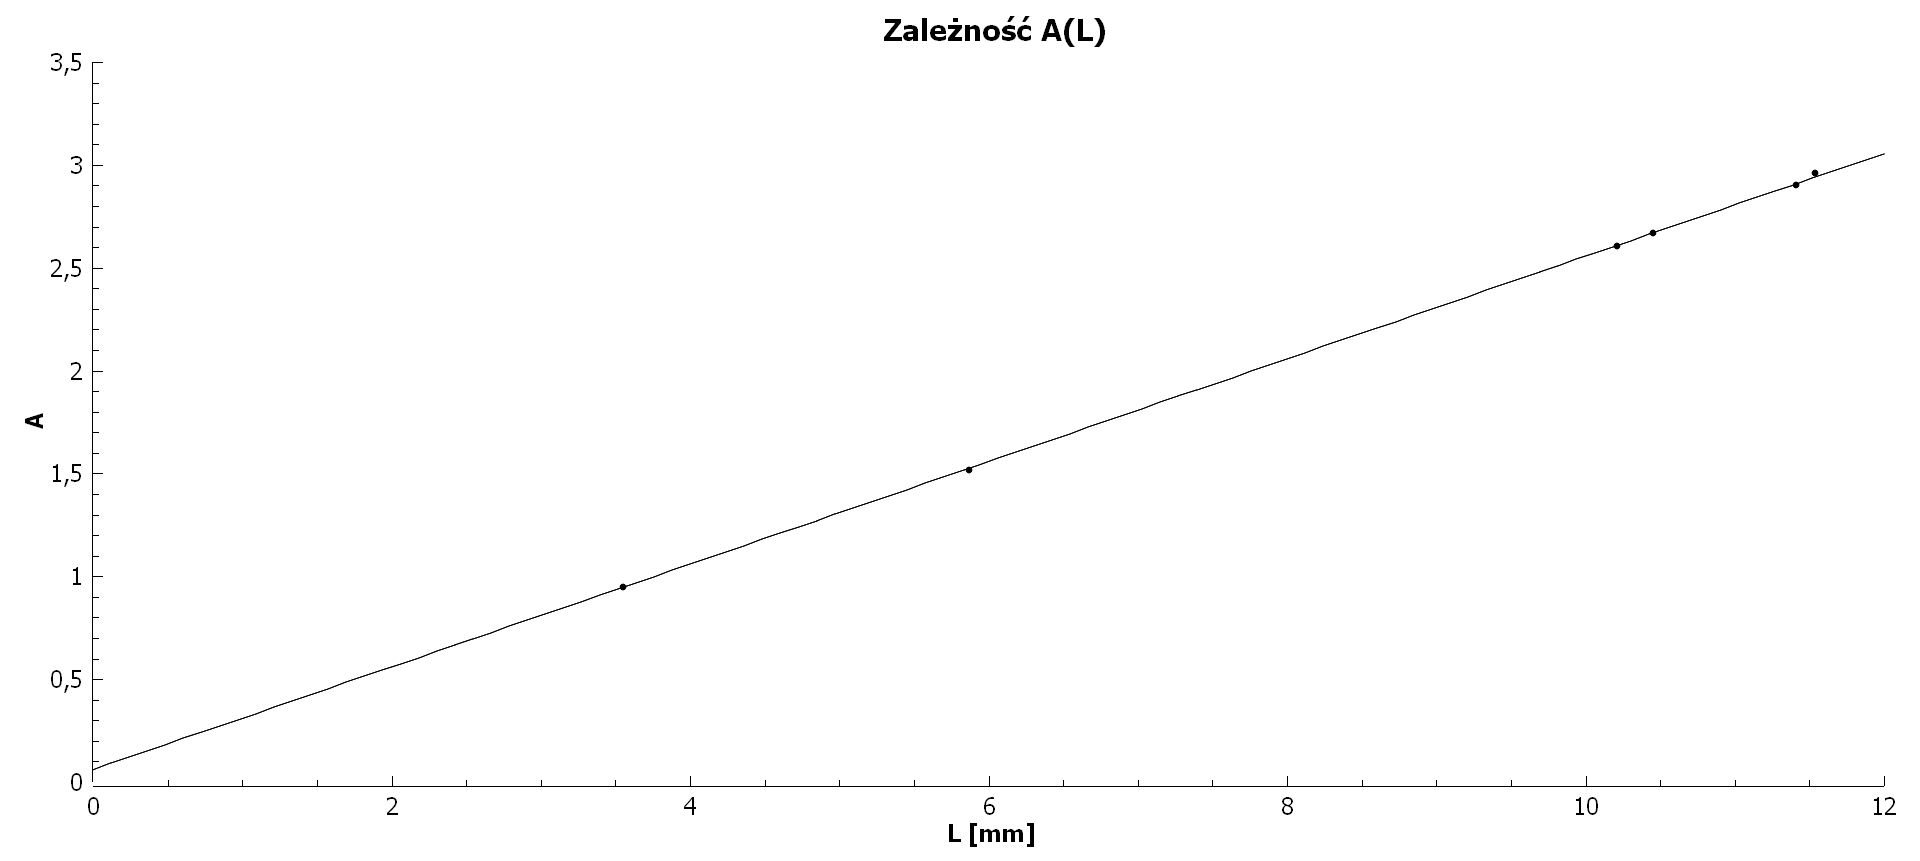
\includegraphics[width=8cm, height=5cm ]{rap72} 
\caption{Zależność A(L) dla dwóch filtrów}
\end{minipage}%
\begin{minipage}{0.5\textwidth}
  \centering
  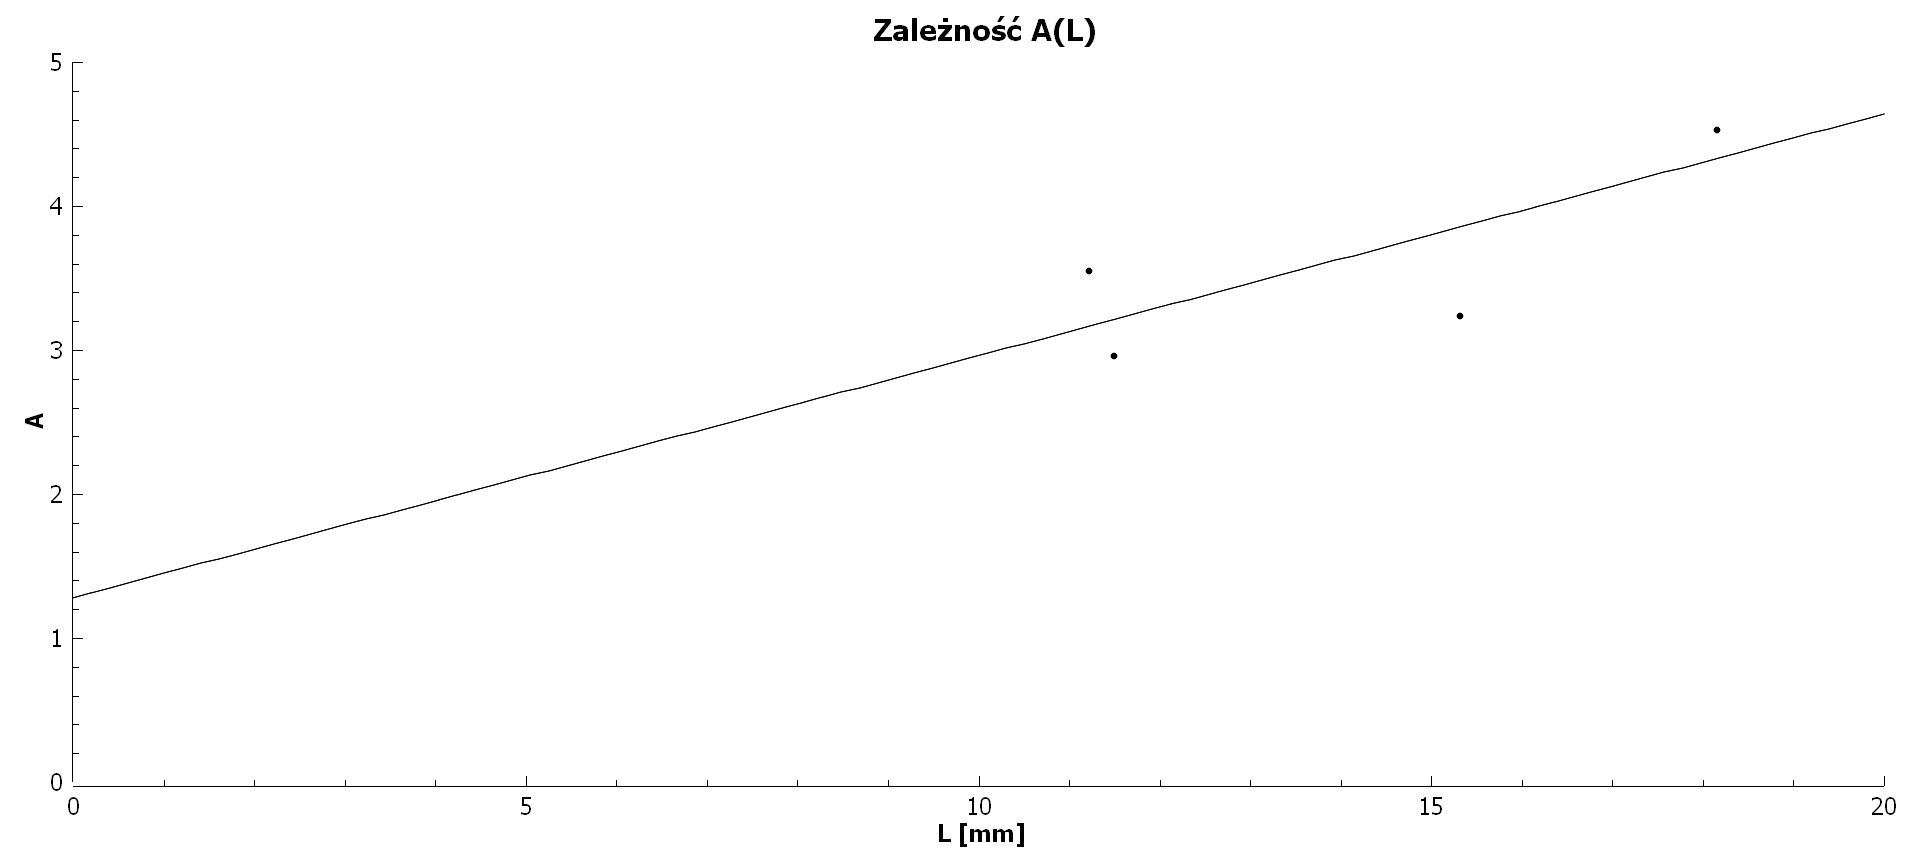
\includegraphics[width=8cm, height=5cm ]{rap73} 
\caption{Zależność A(L) dla trzech filtrów}
\end{minipage}
\end{figure}
 
 
 Analogiczne obliczenia przeprowadzono dla pomiarów ze stężonym roztworem CuSO$_{4}$. W tym przypadku zamiast grubości $L$ występuje wielkość $c$, czyli stężenie danego roztworu. Założono, iż stężenie to jest znane dokładnie. Tabela 9 przedstawia punkty pomiarowe wraz z niepewnościami.
 
 \begin{table}[h!]
\centering
\caption{Tabela pomiarów: roztwór}
\label{t9}
\begin{tabular}{|c|c|c||c|c|c|}
\hline
$c$ [mol/L] & $A$     & $u_{A}$ & $c$ [mol/L] & $A$     & $u_{A}$ \\ \hline
0,00000     & 0,00000 & 0,00000 & 0,57850     & 1,61885 & 0,00461 \\ \hline
0,10518     & 0,34182 & 0,00658 & 0,60605     & 1,69339 & 0,00468 \\ \hline
0,33057     & 0,91278 & 0,00500 & 1,15700     & 2,60507 & 0,00899 \\ \hline
0,38567     & 1,12794 & 0,00556 & 0,89000     & 2,75059 & 0,01122 \\ \hline
0,43388     & 1,23067 & 0,00598 & 0,77133     & 2,17910 & 0,00575 \\ \hline
0,47641     & 1,41318 & 0,00707 & 0,68059     & 2,13198 & 0,00558 \\ \hline
0,51422     & 1,46023 & 0,00746 & 0,60895     & 2,10542 & 0,00549 \\ \hline
0,54805     & 1,50623 & 0,00453 & 0,55095     & 2,06272 & 0,00536 \\ \hline
\end{tabular}
\end{table}
Na potrzeby analizy wykluczono z rozważań punkt o $A=0$, który prowadził do osobliwości. 

Otrzymano $\hat{a}=2,6225\pm0,0080$ L/mol, $\hat{b}=0,1768\pm0,0046$.
Dla takiej liczby punktów pomiarowych $\chi^2= 29,82$. Jednak zgodnie z przeprowadzonymi obliczeniami, $\chi_{0}^2=18820,73$. Tak ogromna wartość z miejsca powoduje odrzucenie wyników, jako nieprawidłowych. Problem wynika z tego, iż w drugiej części pomiarów obluzowało się mocowanie lasera, przez co ten nie trafiał w środek fotodiody. Z tego powodu postanowiono odrzucić wyniki związane z problemami technicznymi. Jednak takie odrzucenie wyników, po uwzględnieniu nowych współczynników, zmniejsza wartość $\chi^2_{0}$ tylko do 299,24. W związku tym postanowiono całkowicie odrzucić wyniki tych pomiarów jako błędne.

Aby wyznaczyć współczynnik absorpcji $\alpha$ postanowiono połączyć współczynniki $\hat{a}$ otrzymane dla analizy z pojedynczym filtrem i dwoma filtrami. Różnica między nimi, wynosząca 0,00174 mm$^{-1}$ nie przekracza wartości $\sigma=0,00185$ niepewności tej różnicy, wyznaczonej na podstawie Równania (7). Tak więc można połączyć ze sobą oba współczynniki korzystając ze średniej ważonej, zdefiniowanej jako:

\begin{equation}
 	\bar{a}_{w}=\dfrac{\sum_{i=1}^{N}\dfrac{a_i}{u_{i}^2}}{\sum_{i=1}^{N}\dfrac{1}{u_{i}^{2}}}.
 	\end{equation}
 Niepewności średniej ważonej wrażają się w następującymi wzorami:
 \begin{eqnarray}
 u^{2}_{int}=\dfrac{1}{\sum_{i=1}^{N}\dfrac{1}{u_{i}^2}}, \\
 u^{2}_{ext}=\dfrac{u_{int}^2}{N-1}\sum_{i=1}^{N}\left(\dfrac{a_{i}-\bar{a}_{w}}{u_{i}}\right)^2.
 \end{eqnarray}
 Jako ostateczną niepewność niepewność wielkości $\bar{a}_{w}$ wybiera się większą z niepewności $u_{int}$ lub $u_{ext}$ \cite{tay4}. 
 
 Podstawienie odpowiednich wartości prowadzi do wyniku $\bar{a}_{w}=0,24906\pm0,00083$ mm$^-1$. Korzystając z zależności, że $\bar{a}_{w}=\alpha\log_{10}(e)$ można wyznaczyć wartość $\alpha$, a korzystając z Równania (7), także jej niepewność.
Otrzymano: $\alpha=0,5735$ mm$^{-1}$, $u_{\alpha}=u_{aw}/\log_{10}(e)=0,0019$ mm$^{-1}$.

Średnia droga swobodna na pochłonięcie fotonu $\lambda$ zdefiniowana jest jako odwrotność współczynnika $\alpha$. Łatwo jest również policzyć jej niepewność: $u_{\lambda}=u_{\alpha}/\alpha^2$. Po podstawieniu wartości liczbowych otrzymano $\lambda=1,7437\pm0,0058$ mm. Otrzymany wynik cechuje się niską niepewnością, wynikłą z dokładnie przeprowadzonych pomiarów i łączenia współczynników.  


\pagebreak


\begin{center}
\textbf{\subsection*{DYSKUSJA WYNIKÓW I WNIOSKI}}
\end{center} 
Wyniki otrzymane dla pomiarów napięcia dla filtrów okazały się być zgodne z przewidywaniami teoretycznymi. Największą niepewnością cechowały się wyniki związanie z trzema filtrami, dlatego też nawet nie brano ich pod uwagę w dalszej części analizy danych. Pozostałe wyniki związane z filtrami cechowały się bardzo dużą dokładnością i pozwoliły na wyznaczenie współczynnika $\alpha$ i $\lambda$ z bardzo małą niepewnością. Niepokojący jest otrzymany wynik dla współczynnika odbicia, a konkretniej jego niepewność, która jest znacznie większa od samego współczynnika. Wynika to prawdopodobnie z malej wartości $R$ samej w sobie, co czyni ją ciężką do zmierzenia metodami pośrednimi.

Najbardziej dotkliwa okazała się strata pomiarów związanych z roztworem CuSO$_{4}$. W tym doświadczeniu, z braku lepszego sprzętu, korzystano z niestabilnego lasera, porysowanej kuwety, czy też strzykawek, które nie pozwalały na płynne dozowanie roztworu. Złożenie tych wszystkich czynników doprowadziło do całkowitej klęski w tej części pomiarowej.


\begin{center}
\begin{thebibliography}{9}

 \bibitem{sz1}
 Sz. Szczeniowski,
 \emph{Fizyka doświadczalna, cz. V, Fizyka atomowa},
 PWN, Warszawa, 1967, s. 28.

 \bibitem{tay1}
 J. R. Taylor,
 \emph{Wstęp do analizy błędu pomiarowego},
 PWN, Warszawa, 1995, s. 175.
 
\bibitem{g1}
  N. W. Smirnow, I. W. Dunin-Barkowski,
  \emph{Kurs rachunku prawdopodobieństwa i statystyki matematycznej dla zastosowań technicznych},
  PWN, Warszawa, 1973, s. 544.
  
   \bibitem{tay3}
 J. R. Taylor,
 \emph{Wstęp do analizy błędu pomiarowego},
 PWN, Warszawa, 1995, s. 251.
 
 \bibitem{tay4}
 J. R. Taylor,
 \emph{Wstęp do analizy błędu pomiarowego},
 PWN, Warszawa, 1995, s. 169. 
  

 
  \end{thebibliography}


\end{center}
\end{document}